\documentclass{article}
\usepackage{amsmath} %Never write a paper without using amsmath for its many new commands
\usepackage{amssymb} %Some extra symbols
\usepackage{makeidx} %If you want to generate an index, automatically
\usepackage{graphicx} %If you want to include postscript graphics
%%%  \usepackage{mystyle}
%Create your own file, mystyle.sty where you put all your own \newcommand statements
%%%
%%%
\usepackage{amscd}

\usepackage{Sweave}


%%\VignetteIndexEntry{Examples from GEOmap}

%%% \usepackage{Sweave}

\begin{document}

%%%\renewcommand\floatpagefraction{.9}
%%%\renewcommand\topfraction{.9}
%%%\renewcommand\bottomfraction{.9}
%%%\renewcommand\textfraction{.1}
%%%\setcounter{totalnumber}{50}
%%%\setcounter{topnumber}{50}
%%%\setcounter{bottomnumber}{50}

\setkeys{Gin}{width=0.9\textwidth}



\numberwithin{equation}{section}

%%%



\author{Jonathan M. Lees\\
University of North Carolina, Chapel Hill\\
Department of Geological Sciences\\
CB \#3315, Mitchell Hall\\
Chapel Hill, NC  27599-3315\\
email: jonathan.lees@unc.edu\\
ph: (919) 962-0695
}
%%  \address{University of North Carolina, Chapel Hill}
%% \contact{Jonathan M. Lees}
%% \contactaddress{Department of Geological Sciences, CB #3315, Mitchell Hall, Chapel Hill, NC  27599-3315}
%% \contactemail{jonathan.lees@unc.edu}
%% \contactphone{(919) 962-0695}
\title{GEOmap: mapping and geology in R}
\date{March , 2008}

\maketitle

\begin{abstract}
Geomap software is aimed at geological applications in mapping. 

\end{abstract}

\section{Introduction}
I developed a set of programs for making complex geological maps in R.
These program parallel, to a certain extent, the maps and the mapdata 
packages already available but they are different in significant ways and 
provide a slightly different set of the utilities.
Maps currently available in the mapdata package can be used
by GEOmap, but most of the data required by 
GEOmap is included in a separate package called geomapdata,
loaded independently. 

The main differences between maps and GEOmap is the lower demands
GEOmap has on requiring the maps information to be stored as independent 
strokes and topologically related polygons.  This step, while useful
and powerful for many applications, is onerous to set up for 
maps that are digitized on the fly, either from paper 
copies or from digital images on the screen.

The other difference is in the handling of projections.  GEOmap
has a few simple cartographic projections built in 
and can be expanded later by users.


\section{Projections}

There are  7 cartographic projections currently installed in 
GEOmap that can be called by the user and applied to data
either in the forward mode (Lat-Lon to x-y) or in the inverse
mode to go from the projected world back to geographic coordinates.

The set up of the projection is accomplished by 
running, for example,

\begin{Schunk}
\begin{Sinput}
> library(GEOmap)
\end{Sinput}
Spatial Point Pattern Analysis Code in S-Plus

 Version 2 - Spatial and Space-Time analysis
GEOmap is loaded\begin{Sinput}
> options(continue = " ")
> kliuLL = c(56.056, 160.64)
> PROJ = setPROJ(type = 2, LAT0 = kliuLL[1], LON0 = kliuLL[2], 
     LATS = NULL, LONS = NULL, DLAT = NULL, DLON = NULL, FN = 0)
\end{Sinput}
\end{Schunk}

This makes this location (Kliuchevskoi volcano in Kamchatka, Russia) the origin 
of a utm spherical projection.
The structure PROJ must be passed as an argument to subsequent 
calls to GEOmap plotting routines and conversions.
The choices for projections can be seen by calling  projtype()
as in,
\begin{Schunk}
\begin{Sinput}
> projtype()
\end{Sinput}
\begin{Soutput}
[1] Projection Types
[1] 0 = None
[1] 1 = merc.sphr
[1] 2 = utm.sphr
[1] 3 = lambert.cc
[1] 4 = stereo.sphr
[1] 5 = utm.elps
[1] 6 = equid.cyl
[1] 99 = old crosson projection
\end{Soutput}
\end{Schunk}

And we can see the usage of the projection by loading and plotting a map.
First we plot the map with no projection, so the xy coordinates are Lat-Lon
and the map will be distorted.

\begin{Schunk}
\begin{Sinput}
> require("geomapdata")
> data(kammap)
> plotGEOmap(kammap, add = FALSE, asp = 1)
\end{Sinput}
\end{Schunk}
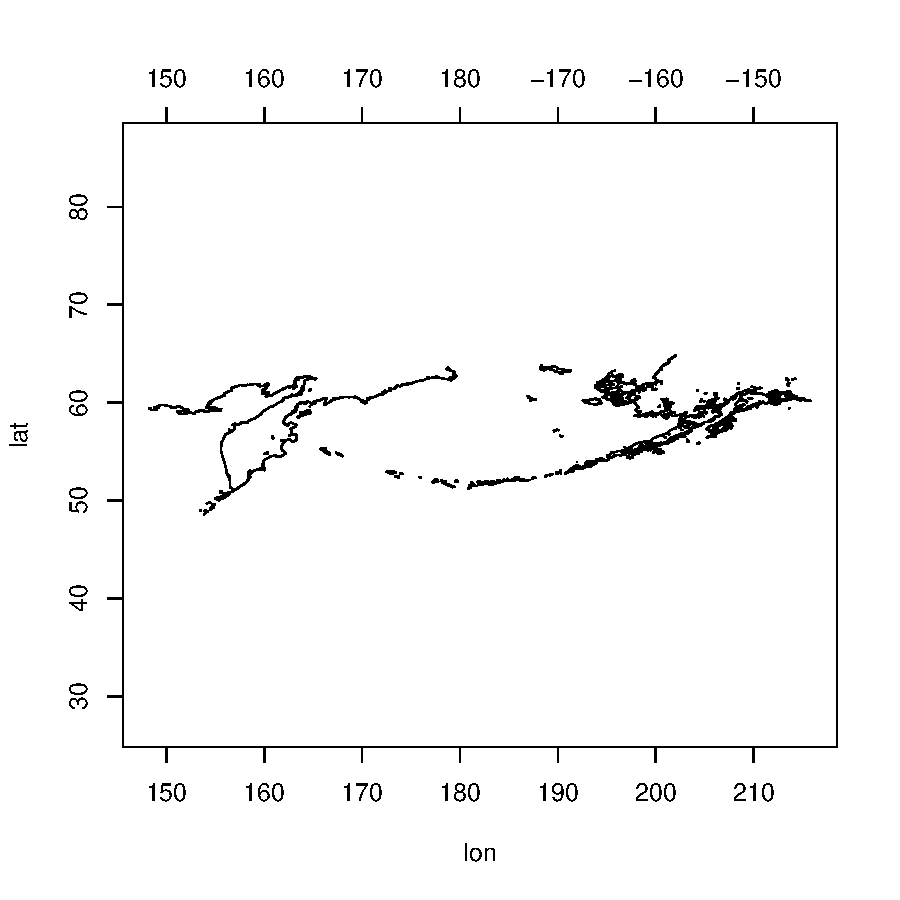
\includegraphics{gmap-003}

Next we show how to plot the map in projected form,
\begin{Schunk}
\begin{Sinput}
> plotGEOmapXY(kammap, PROJ = PROJ, add = FALSE, xlab = "km", ylab = "km")
\end{Sinput}
\end{Schunk}
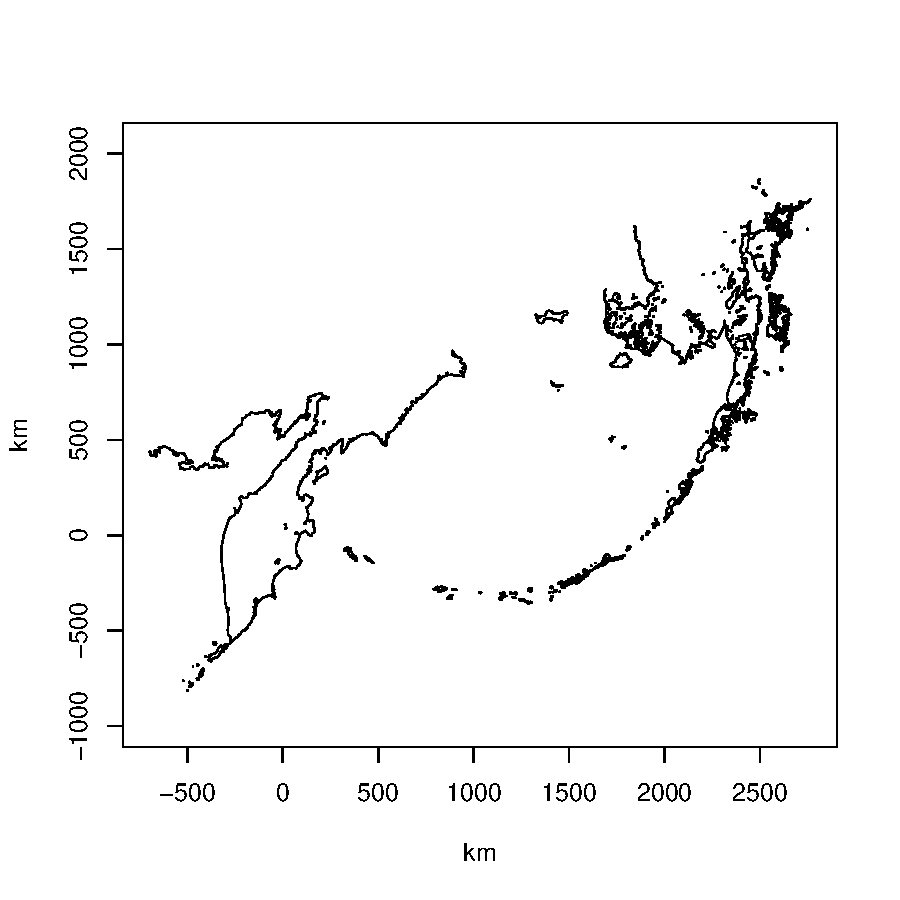
\includegraphics{gmap-004}

Notice that by resizing the window the map retains the proper
aspect ration and the units are correct.

\section{Simple Map}

\section{Map Structure}

The internal structure of a GEOmap objection consists of
three elements which are lists themselves.
The raw XY coordinates are stored as long vectors
on the POINTS list.  These are all the geographic coordinates of the 
points int he map structure.  
The STROKES structure contains the meta data that allows one to 
access the POINTS and perform tasks and create graphical output.
The STROKES structure includes a set of vectors which have the following structure:

\section{Geologic Example}

The following illustrates some of the features available in GEOmap.
First we set up the data and then begin making the plot after manipulating the 
database.

\begin{Schunk}
\begin{Sinput}
> data(cosomap)
> data(faults)
> data(hiways)
> data(owens)
> data(cosogeol)
> proj = cosomap$PROJ
> plotGEOmapXY(cosomap, PROJ = proj, add = FALSE, ann = FALSE, 
     axes = FALSE)
> cosogeol = boundGEOmap(cosogeol)
> plotGEOmapXY(cosogeol, PROJ = proj, add = TRUE, ann = FALSE, 
     axes = FALSE)
> plotGEOmapXY(cosomap, PROJ = proj, add = TRUE, ann = FALSE, axes = FALSE)
> plotGEOmapXY(faults, PROJ = proj, add = TRUE, ann = FALSE, axes = FALSE)
\end{Sinput}
\end{Schunk}
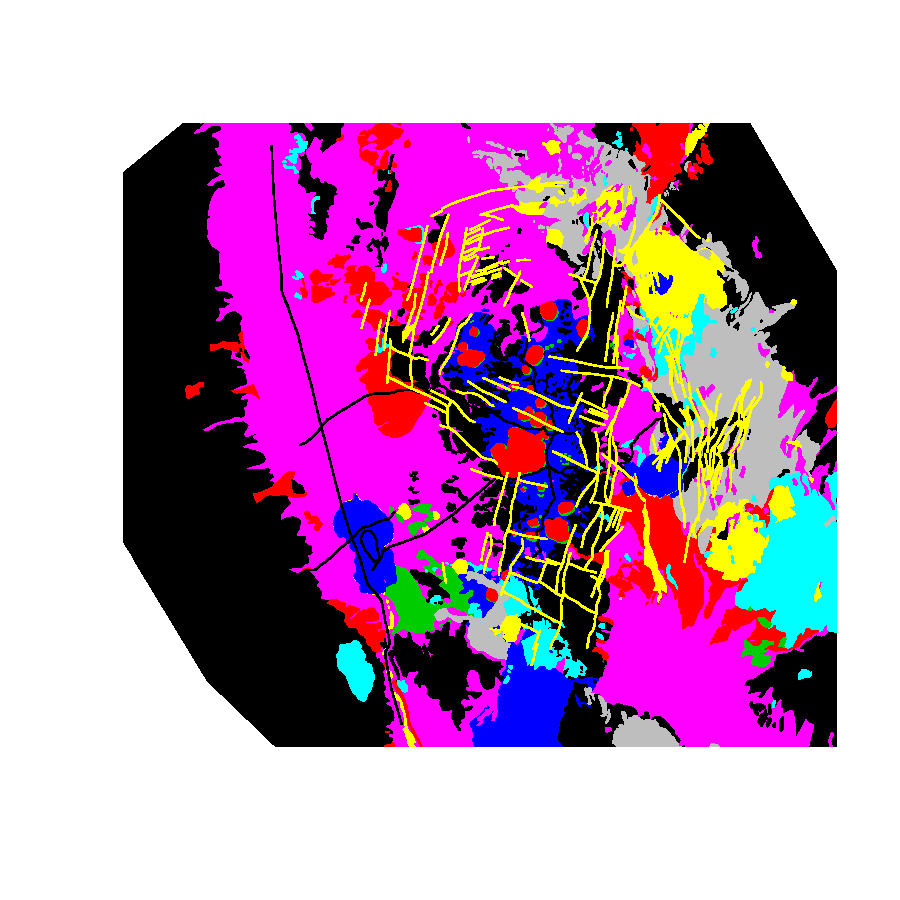
\includegraphics{gmap-005}

The colors here are not very useful, so we can modify them by
assigning colors from a given palette, in this case
the palette of the program geotouch,
\begin{Schunk}
\begin{Sinput}
> XMCOL = setXMCOL()
> cosocolnumbers = 1:length(cosogeol$STROKES$col)
> newcol = XMCOL[cosogeol$STROKES$col]
> cosocolnums = cosogeol$STROKES$col
> cosogeol$STROKES$col = newcol
\end{Sinput}
\end{Schunk}
and lastly we must create a legend by matching the colors with the
symbols or names of hte units:
\begin{Schunk}
\begin{Sinput}
> ss = strsplit(cosogeol$STROKES$nam, split = "_")
> geo = unlist(lapply(ss, FUN = "getmem", mem = 1))
> UGEO = unique(geo)
> mgeo = match(geo, UGEO)
> cosogeol = boundGEOmap(cosogeol)
> gcol = paste(sep = ".", geo, cosogeol$STROKES$col)
> ucol = unique(gcol)
> spucol = strsplit(ucol, split = "\\.")
> N = length(spucol)
> names = unlist(lapply(spucol, FUN = "getmem", mem = 1))
> shades = unlist(lapply(spucol, FUN = "getmem", mem = 2))
> ORDN = order(names)
> plotGEOmapXY(cosomap, PROJ = proj, add = FALSE, ann = FALSE, 
     axes = FALSE)
> plotGEOmapXY(cosogeol, PROJ = proj, add = TRUE, ann = FALSE, 
     axes = FALSE)
> plotGEOmapXY(cosomap, PROJ = proj, add = TRUE, ann = FALSE, axes = FALSE)
> plotGEOmapXY(faults, PROJ = proj, add = TRUE, ann = FALSE, axes = FALSE)
> geoLEGEND(names[ORDN], shades[ORDN], 0.28, 0.14, 16, 6)
\end{Sinput}
\end{Schunk}
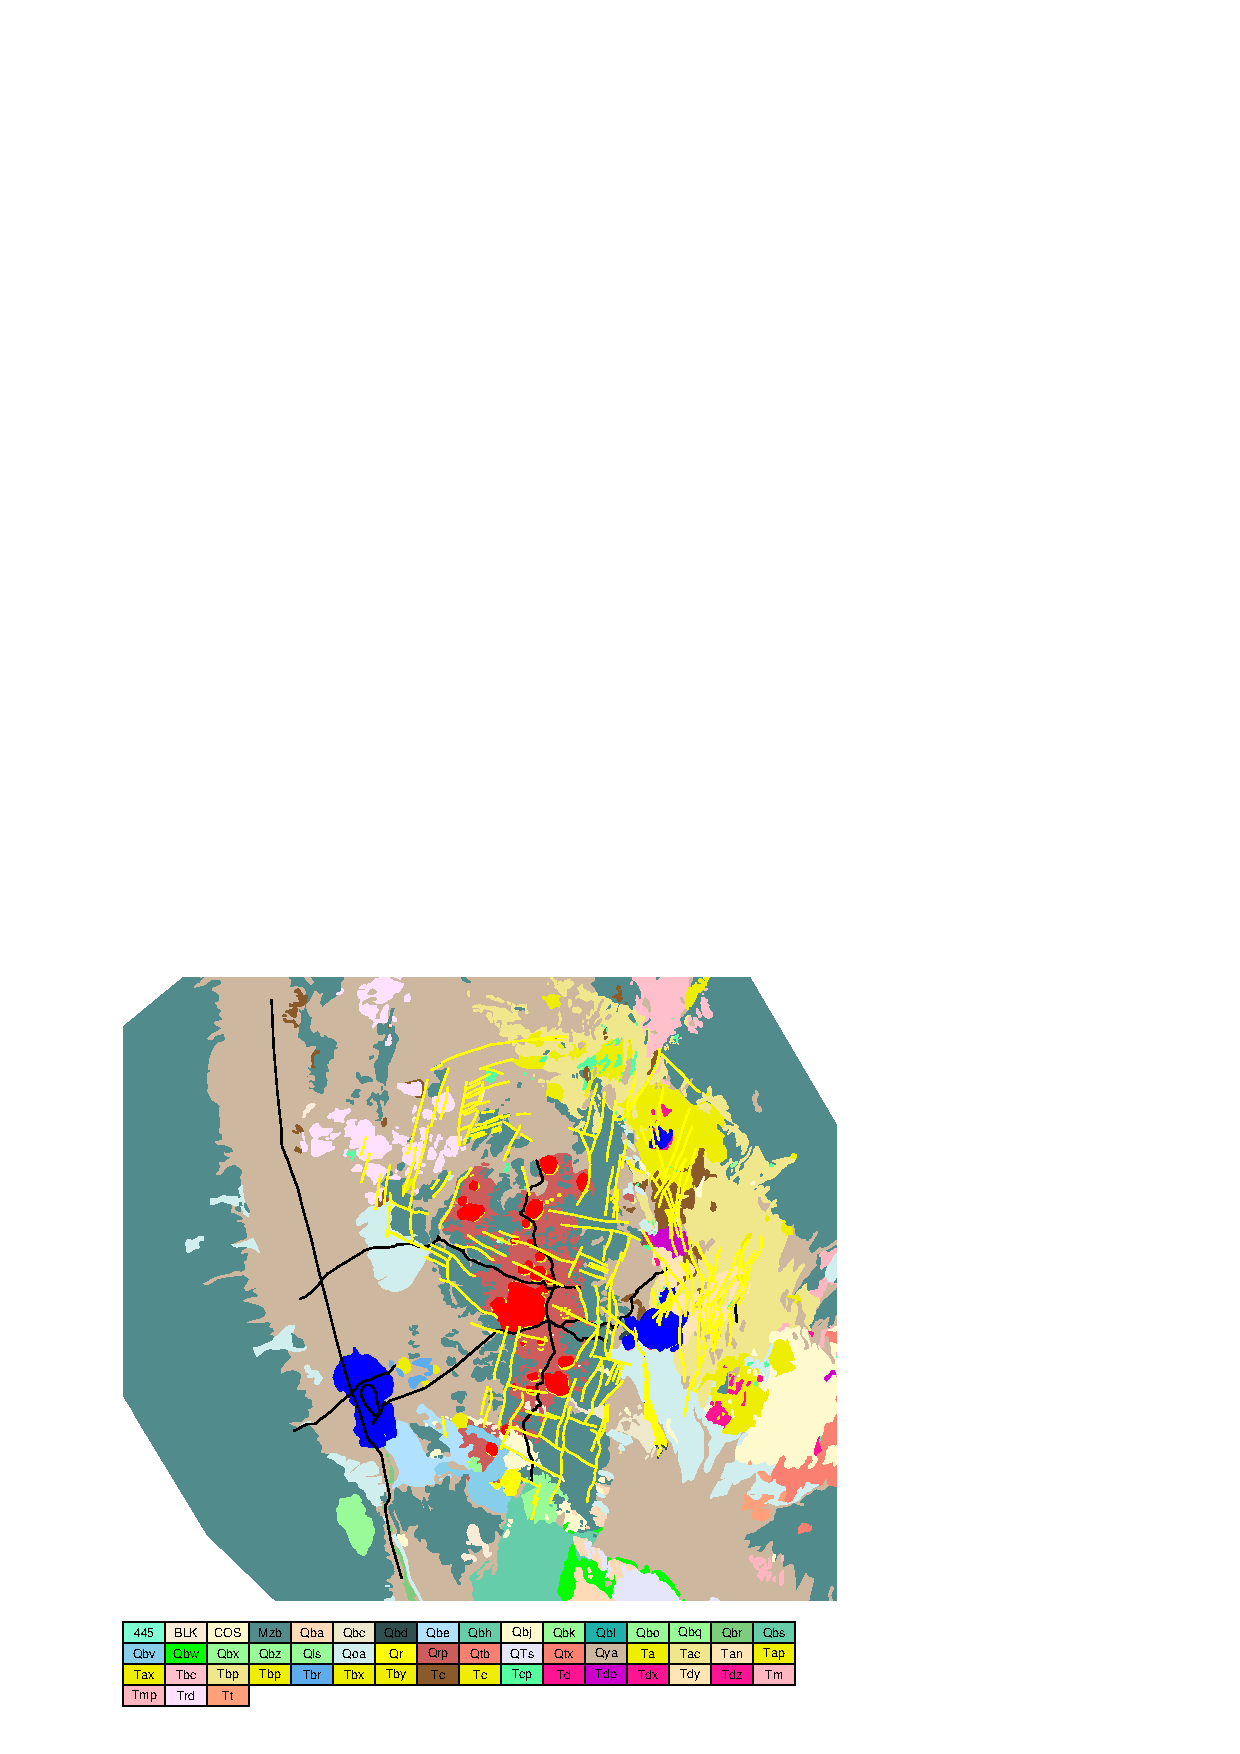
\includegraphics{gmap-007}


\section{Building a map plot and controling the figure}


In this section I illustrate how to build a map figure by adding several components,
and controlling the plotting functions.
We start by first reading in some data.  
The volcano data is taken from the Smithsonian Institution web site
listing volcanoes of the world.  These have been converted to s simple 
file including LAT, LON, Elevation and volcano name.
The station represent the station locations for
the NIED network in Japan.
The earthquakes are taken from a catalog of earthquake hypocenters
that can be downloaded from the Internet from a variety of 
websites currently available.

\begin{Schunk}
\begin{Sinput}
> jvolcs = scan(file = "Volc_points.LLZ", what = list(name = "", 
     lat = 0, lon = 0, h = 0), sep = " ")
> stas = scan(file = "newFUJIstation.LLZ", what = list(name = "", 
     lat = 0, lon = 0, h = 0), sep = " ")
> eqs = scan(file = "japan.eng", what = list(lon = 0, lat = 0, 
     z = 0, m = 0))
\end{Sinput}
\end{Schunk}

Next we set the projection to be centered on Mt. Fuji 
with a UTM projection.
To extract the LAT-LON of Mt. Fuji from the volcano
data base, we use the grep function to match 
the character string FUJI with the corresponding name in the data set.


\begin{Schunk}
\begin{Sinput}
> ifuji = grep("FUJI", jvolcs$name)
> PROJ = setPROJ(type = 2, LAT0 = jvolcs$lat[ifuji], LON0 = jvolcs$lon[ifuji])
\end{Sinput}
\end{Schunk}

We load up the japmap provided by the geomapdata package,
create the projected plot and limit the plotting region
to a LAT-LON rectangle described by the vector FUJIAREA.
This is calculated using the XY.GLOB function that takes x-y 
coordinates in km and converts to LAT-LON geographic coordinates.
These are stored in vector FUJIAREA as
a rectangular region, and used in plotGEOmapXY
to restrict the plotting region.  Here we have 
used a distance of 15o km north and south of
Mt. Fuji as our target region.

\begin{Schunk}
\begin{Sinput}
> LL = XY.GLOB(c(-150, 150), c(-150, 150), PROJ = PROJ)
> FUJIAREA = c(LL$lon[1], LL$lat[1], LL$lon[2], LL$lat[2])
\end{Sinput}
\end{Schunk}

Now we are ready to plot the data previously
scanned and add to the current plot using the same
projection parameters stored in list PROJ.
First the whole of Japan is plotted 
with the volcanoes plotted as triangle.

\begin{Schunk}
\begin{Sinput}
> require("geomapdata")
> data("japmap", package = "geomapdata")
> plotGEOmapXY(japmap, PROJ = PROJ, xlab = "km", ylab = "km")
> pointsGEOmapXY(jvolcs$lat, jvolcs$lon, PROJ = PROJ, col = "red", 
     pch = 2, cex = 0.5)
> rect(-150, -150, 150, 150)
\end{Sinput}
\end{Schunk}
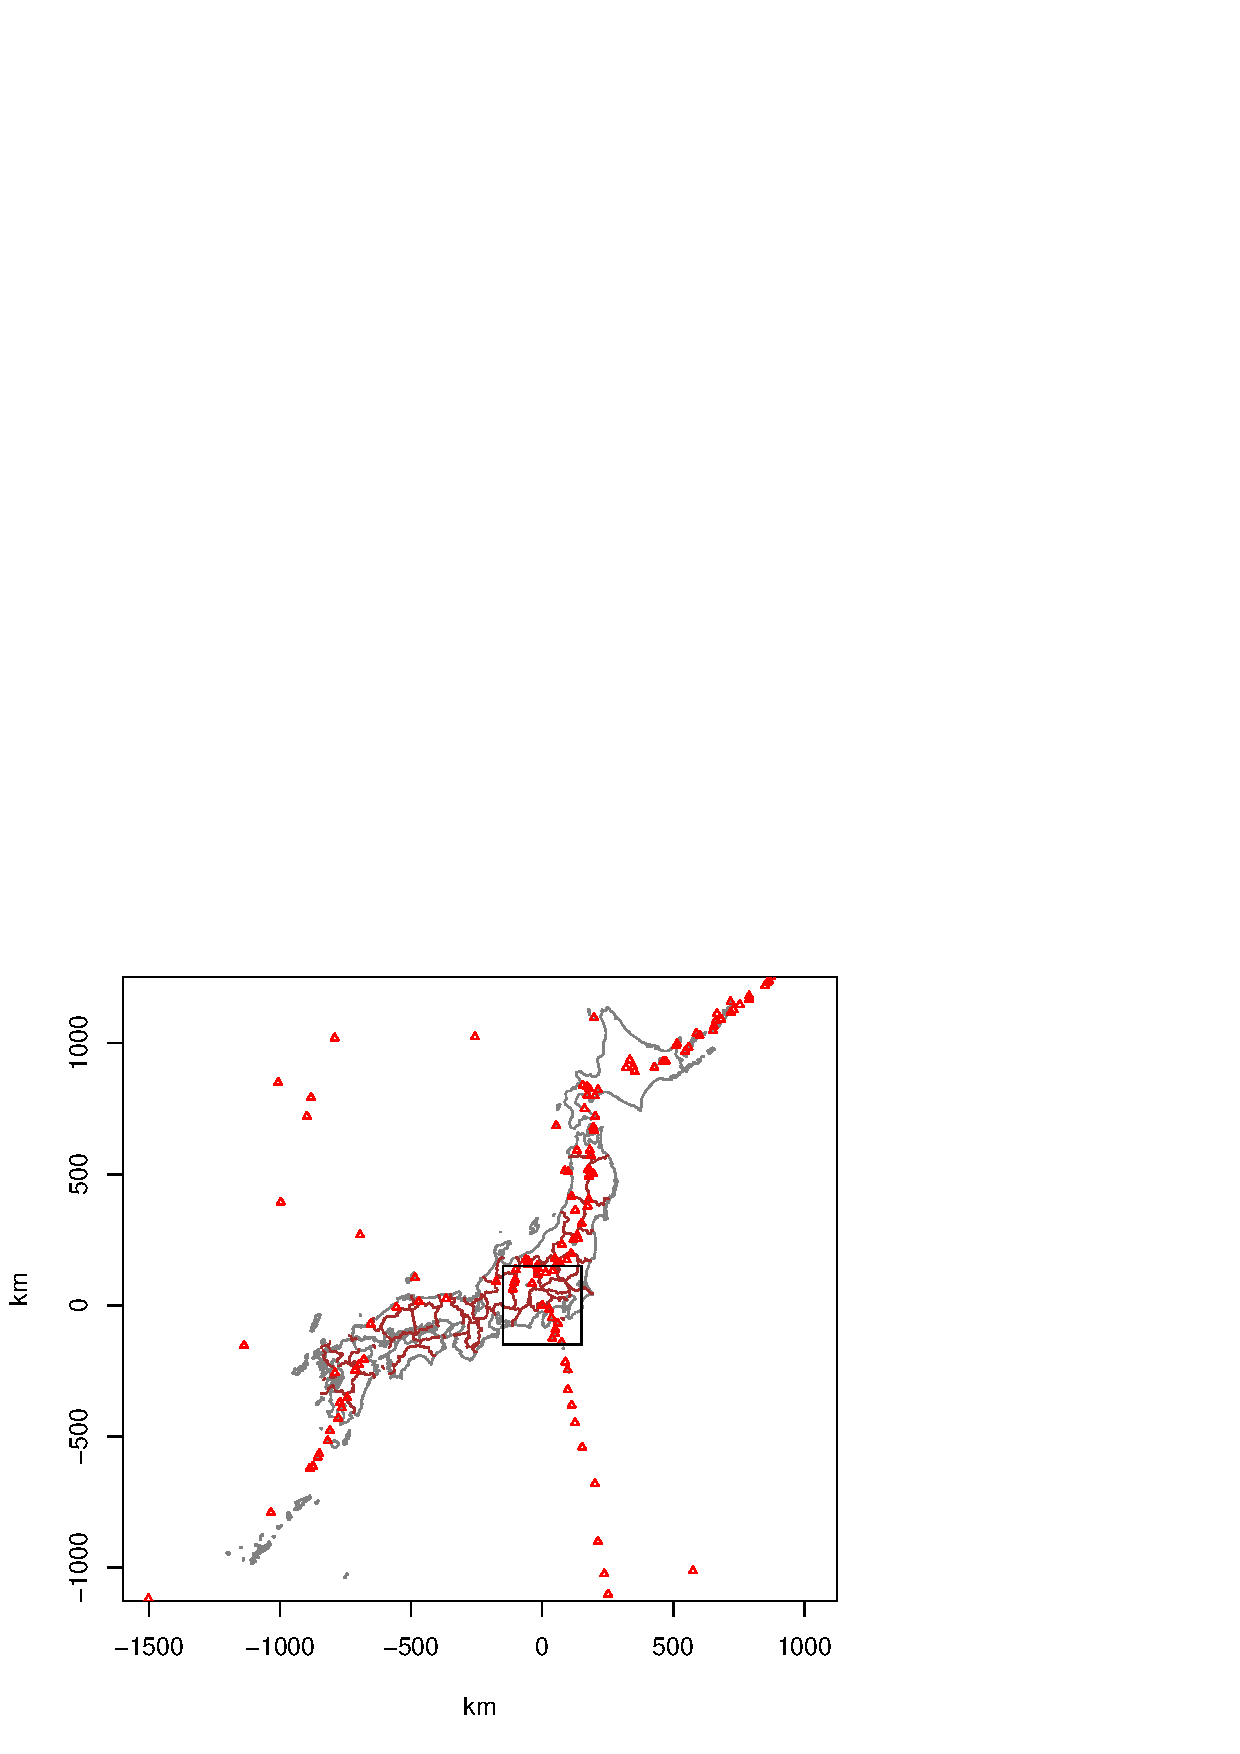
\includegraphics{gmap-011}

Next we can zoom into the desired target region shown as a rectangle 
in the previous figure:

\begin{Schunk}
\begin{Sinput}
> plotGEOmapXY(japmap, LIM = FUJIAREA, PROJ = PROJ, xlab = "km", 
     ylab = "km")
> pointsGEOmapXY(jvolcs$lat, jvolcs$lon, PROJ = PROJ, col = "red", 
     pch = 2, cex = 0.5)
> textGEOmapXY(jvolcs$lat, jvolcs$lon, PROJ = PROJ, labels = jvolcs$name, 
     cex = 0.5, pos = 3)
\end{Sinput}
\end{Schunk}
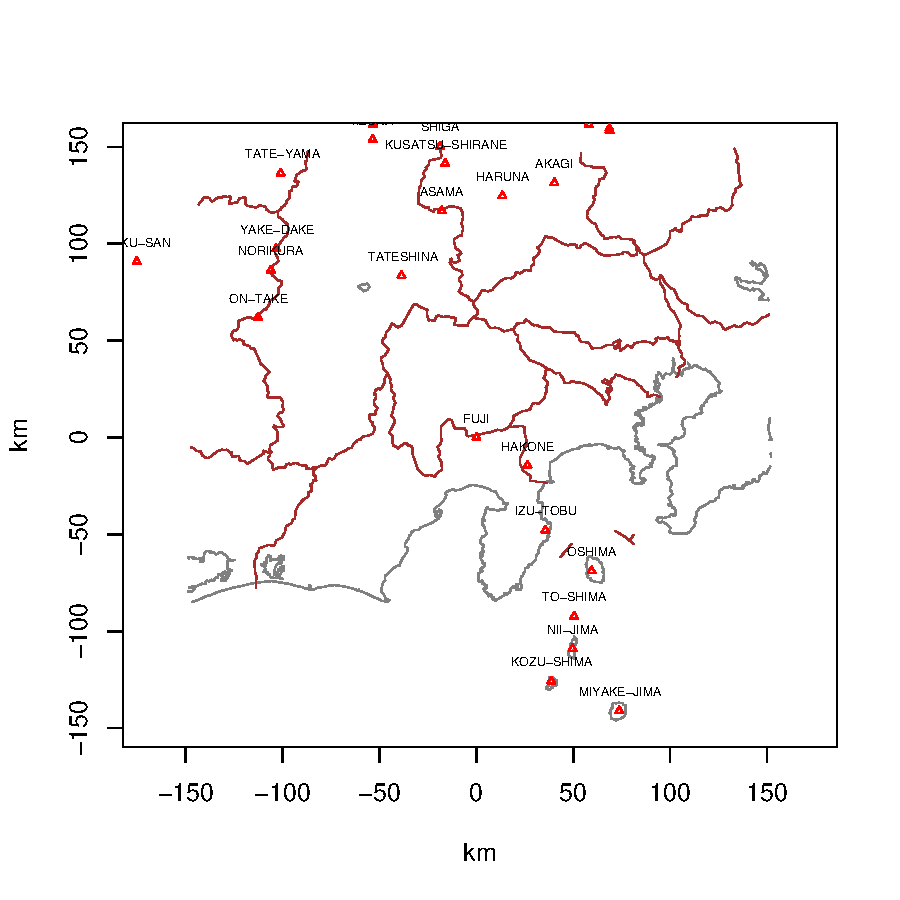
\includegraphics{gmap-012}


To restrict plotting of specific 
features in the map database japmap we can 
pass a selection vector to the 
plotting program.  In this case the Japan 
map has coastal data and internal prefecture boundaries.
The prefecture boundaries are useful for
orientation on maps, but they may also clutter a
plot if they are not needed.
In this case the STROKES in the data 
have tags labeled either ``a'' or ``i'', where the tag
``i'' stands for internal.

\begin{Schunk}
\begin{Sinput}
> print(japmap$STROKES$code)
\end{Sinput}
\begin{Soutput}
  [1] "a" "a" "a" "a" "a" "a" "a" "a" "a" "a" "a" "a" "a" "a" "a" "a" "a" "a"
 [19] "a" "a" "a" "a" "a" "a" "a" "a" "a" "a" "a" "a" "a" "a" "a" "a" "a" "a"
 [37] "a" "a" "a" "a" "a" "a" "a" "a" "a" "a" "a" "a" "a" "a" "a" "a" "a" "a"
 [55] "a" "a" "a" "a" "a" "a" "a" "a" "a" "a" "a" "a" "a" "a" "a" "a" "a" "a"
 [73] "a" "a" "a" "a" "a" "a" "a" "a" "a" "a" "a" "a" "a" "a" "a" "a" "a" "a"
 [91] "a" "a" "a" "a" "a" "a" "a" "a" "a" "a" "a" "a" "a" "a" "a" "a" "a" "a"
[109] "a" "a" "a" "a" "a" "a" "a" "a" "a" "a" "a" "a" "a" "a" "a" "a" "a" "a"
[127] "a" "a" "a" "a" "a" "a" "a" "a" "a" "a" "a" "a" "a" "a" "a" "a" "a" "a"
[145] "a" "a" "a" "i" "i" "i" "i" "i" "i" "i" "i" "i" "i" "i" "i" "i" "i" "i"
[163] "i" "i" "i" "i" "i" "i" "i" "i" "i" "i" "i" "i" "i" "i" "i" "i" "i" "i"
[181] "i" "i" "i" "i" "i" "i" "i" "i" "i" "i" "i" "i" "i" "i" "i" "i" "i" "i"
[199] "i" "i" "i" "i" "i" "i" "i" "i" "i" "i" "i" "i" "i" "i" "i" "i" "i"
\end{Soutput}
\end{Schunk}

if we choose those strokes that are not internal 
and create a selection vector, we can quickly elliminate 
the internal boundaries.

\begin{Schunk}
\begin{Sinput}
> isel = which(japmap$STROKES$code != "i")
> plotGEOmapXY(japmap, LIM = FUJIAREA, PROJ = PROJ, SEL = isel, 
     xlab = "km", ylab = "km")
> pointsGEOmapXY(jvolcs$lat, jvolcs$lon, PROJ = PROJ, col = "red", 
     pch = 2, cex = 0.5)
> textGEOmapXY(jvolcs$lat, jvolcs$lon, PROJ = PROJ, labels = jvolcs$name, 
     cex = 0.5, pos = 3)
\end{Sinput}
\end{Schunk}
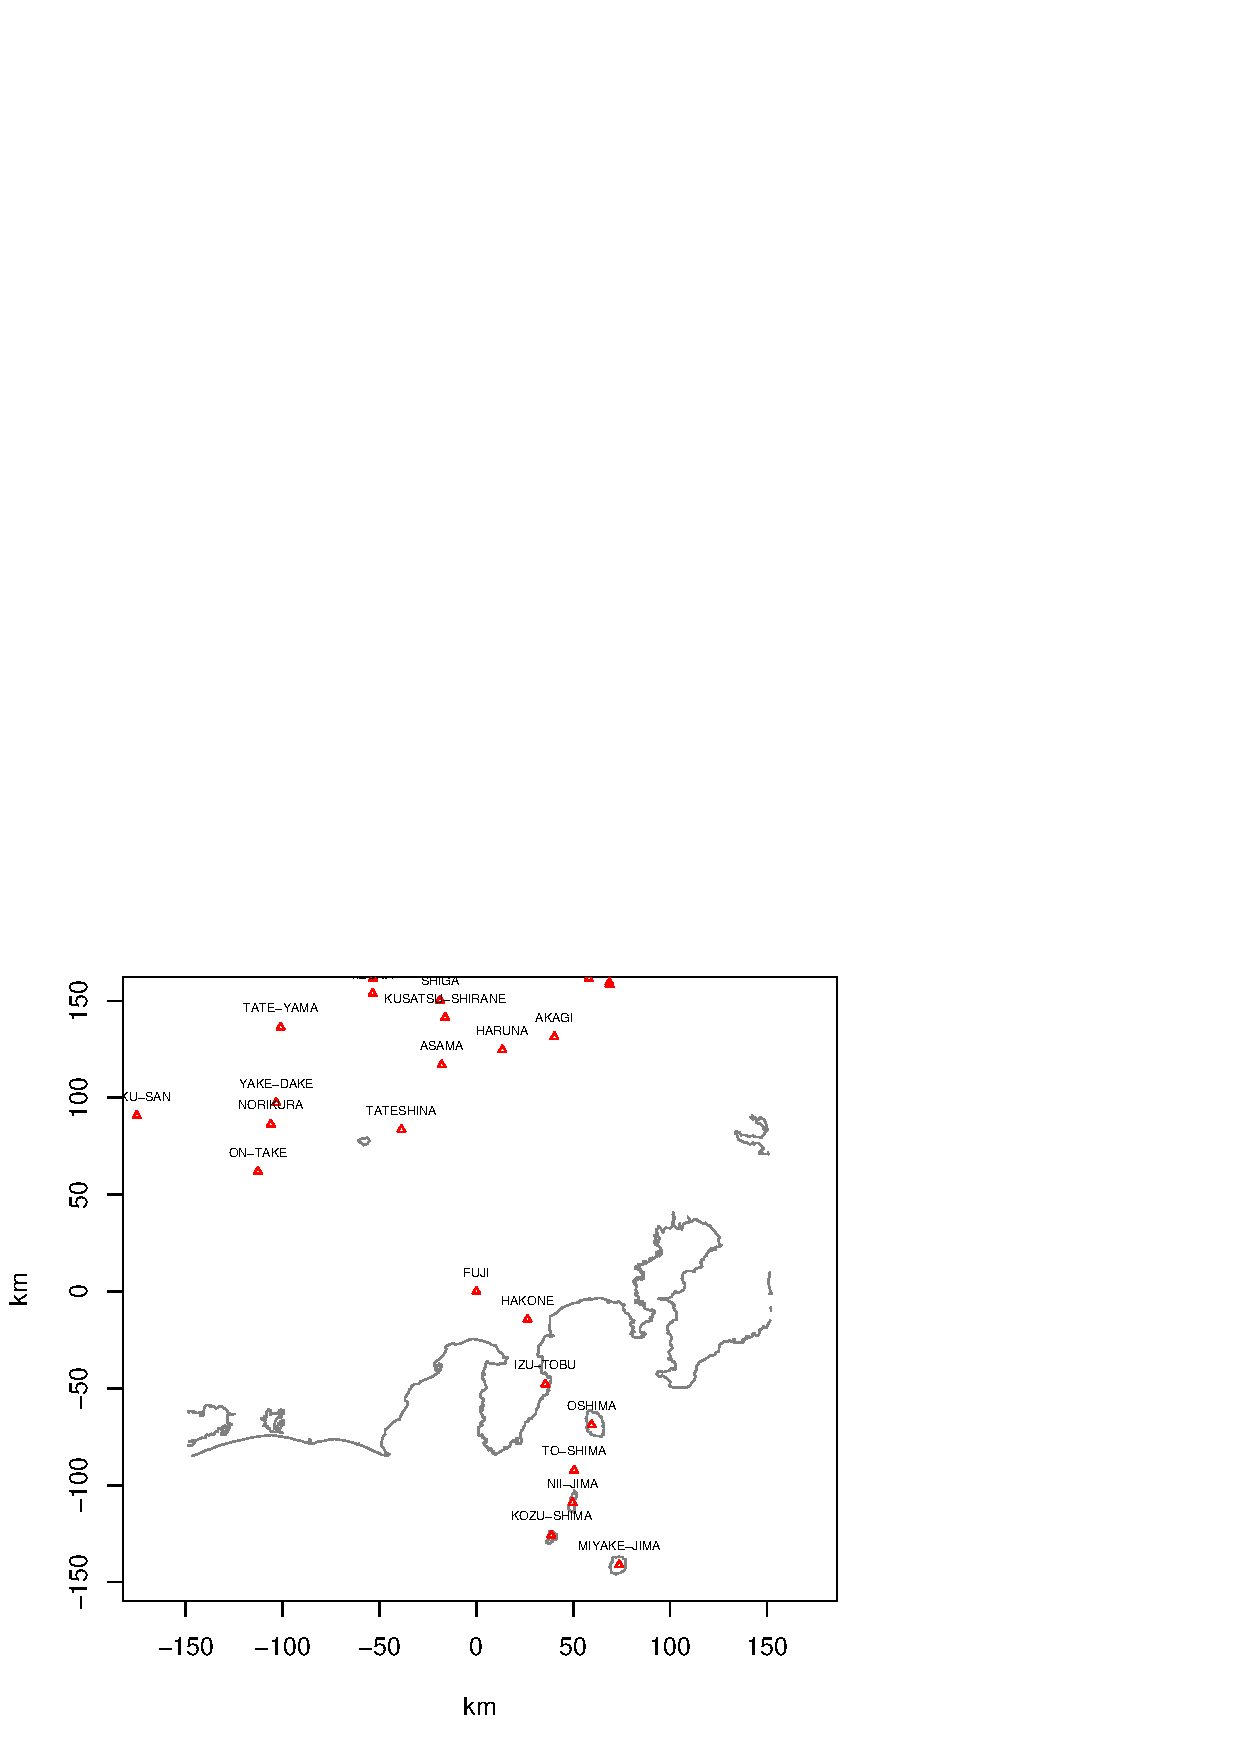
\includegraphics{gmap-014}

\section{Convert from a GMT file}

Many earth scientists use the program GMT (Generic Mapping Tools)
 to make figures for research and publication.  
GMT is a program that includes plotting routines, a small amount of analysis and
numerous cartographic projections.  The main output of GMT is postscript 
figures.  One purpose of GEOmap is to replace GMT with a more general mapping platform
that produces figures as well is high level statistical analysis.

As a result I show here how one can convert a file used by GMT to a GEOmap data file.
Map information in GMT are stored 
as strokes separated by a flagged marker, typically 
by the greater than symbol ``>''.
Here we read in a GMT map file that 
has coordinates of the crude, world, plate-tectonic boundaries. 

\begin{Schunk}
\begin{Sinput}
> plates = scan(file = "Plates.gmt", what = "", sep = "\n")
\end{Sinput}
\end{Schunk}

This file has separated strokes, but also some more information (meta data) 
on the separator lines,
which can be used to augment the GEOmap database.
There are 89 strokes in this data file.  These are the first 
10 headers:

\begin{Schunk}
\begin{Sinput}
> g = grep("^>", plates)
> plates[g[1:10]]
\end{Sinput}
\begin{Soutput}
 [1] "> PLT1 13 2 13 p 3.800000 12.500000 93.599998 91.800003"     
 [2] "> PLT2 35 2 13 p -9.400000 2.900000 114.900002 94.500000"    
 [3] "> PLT3 16 2 13 p 53.090000 59.124100 -142.994995 -164.031006"
 [4] "> PLT4 7 2 13 p 50.610699 52.518600 -165.889999 -178.641998" 
 [5] "> PLT5 12 2 13 p 50.633400 55.190498 179.565002 163.968994"  
 [6] "> PLT6 4 2 13 p -10.300000 -9.500000 122.400002 116.400002"  
 [7] "> PLT7 32 2 13 p 1.900000 34.500000 138.300003 121.599998"   
 [8] "> PLT8 11 2 13 p -1.200000 1.200000 136.500000 131.000000"   
 [9] "> PLT9 8 2 13 p 17.000000 20.000000 94.099998 93.800003"     
[10] "> PLT10 23 2 13 p 3.100000 34.000000 147.300003 132.100006"  
\end{Soutput}
\end{Schunk}

First we will read in each stroke, extract the LAT-LON
information and store in a list.
\begin{Schunk}
\begin{Sinput}
> PLATES = list(STROKES = list(nam = NULL, num = NULL, index = NULL, 
     col = NULL, style = NULL, code = NULL), POINTS = list(lat = NULL, 
     lon = NULL))
> K = 0
> for (i in 1:length(g)) {
     i1 = g[i] + 1
     i2 = g[i + 1] - 1
     if (i == length(g)) 
         i2 = length(plates)
     LONLAT = as.numeric(unlist(strsplit(plates[i1:i2], split = " ")))
     lon = LONLAT[seq(from = 1, to = length(LONLAT), by = 2)]
     lat = LONLAT[seq(from = 2, to = length(LONLAT), by = 2)]
     PLATES$POINTS$lat = c(PLATES$POINTS$lat, lat)
     PLATES$POINTS$lon = c(PLATES$POINTS$lon, lon)
     PLATES$STROKES$nam = c(PLATES$STROKES$nam, paste("PLATE", 
         i, sep = ""))
     PLATES$STROKES$num = c(PLATES$STROKES$num, length(lat))
     PLATES$STROKES$index = c(PLATES$STROKES$index, K)
     PLATES$STROKES$col = c(PLATES$STROKES$col, "blue")
     PLATES$STROKES$style = c(PLATES$STROKES$style, 2)
     PLATES$STROKES$code = c(PLATES$STROKES$code, "p")
     K = K + length(lat)
 }
> PLATES$POINTS$lon = fmod(PLATES$POINTS$lon, 360)
> PLATES = boundGEOmap(PLATES, NEGLON = FALSE)
> PLATES$PROJ = PROJ
\end{Sinput}
\end{Schunk}
\begin{Schunk}
\begin{Sinput}
> data(worldmap)
> plotGEOmap(worldmap, asp = 1)
> plotGEOmap(PLATES, add = TRUE)
\end{Sinput}
\end{Schunk}
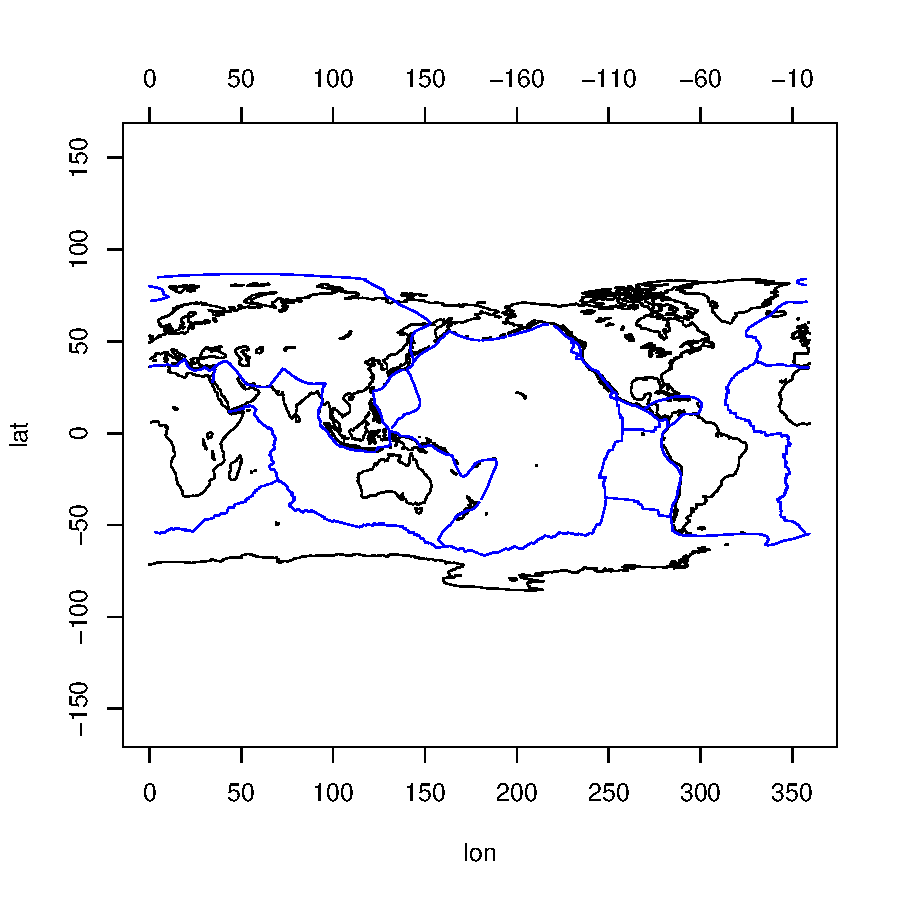
\includegraphics{gmap-018}

Or to show the map of Japan, projected with volcanoes, earthquakes and plate tectonic boundaries, 

\begin{Schunk}
\begin{Sinput}
> plotGEOmapXY(japmap, PROJ = PROJ, SEL = isel, xlab = "km", ylab = "km")
> pointsGEOmapXY(jvolcs$lat, jvolcs$lon, PROJ = PROJ, col = "red", 
     pch = 2, cex = 0.5)
> pointsGEOmapXY(eqs$lat, eqs$lon, PROJ = PROJ, col = "green", 
     pch = ".", cex = 2)
> plotGEOmapXY(PLATES, PROJ = PROJ, add = TRUE)
\end{Sinput}
\end{Schunk}
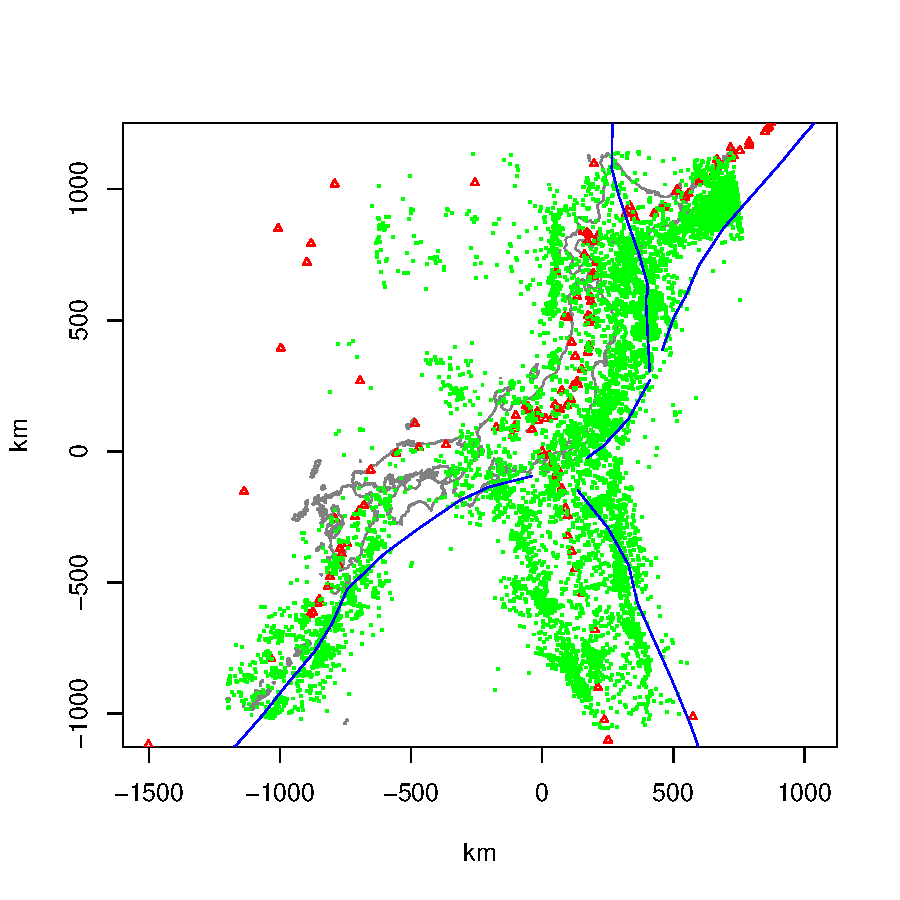
\includegraphics{gmap-019}

Here the earthquakes are plotted as one single color but often
we would like to see the 
events plotted with colors coded according to 
depth,


\begin{Schunk}
\begin{Sinput}
> rcol = rainbow(120)
> ecol = 1 + floor(99 * (eqs$z - min(eqs$z))/(max(eqs$z) - min(eqs$z)))
> plotGEOmapXY(japmap, PROJ = PROJ, SEL = isel, xlab = "km", ylab = "km")
> pointsGEOmapXY(eqs$lat, eqs$lon, PROJ = PROJ, pch = ".", cex = 2, 
     col = rcol[ecol])
> plotGEOmapXY(PLATES, PROJ = PROJ, add = TRUE)
\end{Sinput}
\end{Schunk}
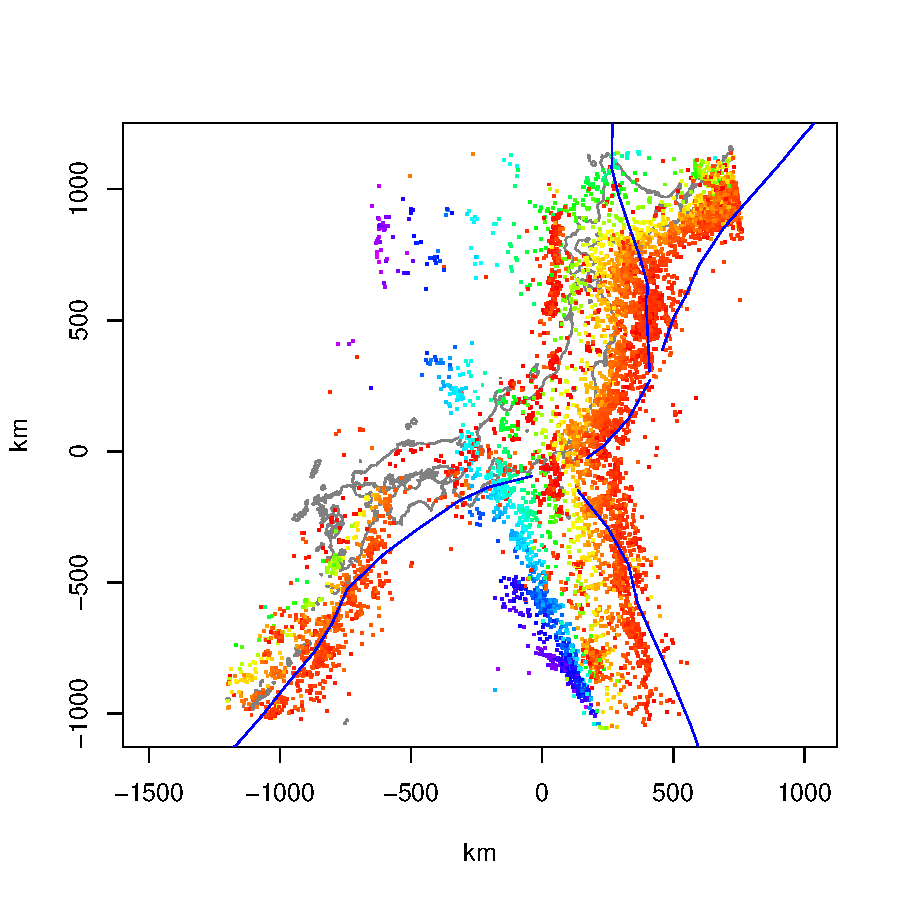
\includegraphics{gmap-020}

To finish off the plot we had the horizontal scale in km, the
size of the earthquakes scaled by magnitude with a small legend at the top,
and a horzontal scale showing the colors associated with depth.
The following is a short function for plotting the 
earthquake size scale at the top.
\begin{Schunk}
\begin{Sinput}
> print(sizelegend)
\end{Sinput}
\begin{Soutput}
function (se, am, pch = pch) 
{
    if (missing(pch)) 
        pch = 1
    u = par("usr")
    ex = c(u[1] + 0.05 * (u[2] - u[1]), u[1] + 0.2 * (u[2] - 
        u[1]))
    why = u[3] + 0.95 * (u[4] - u[3])
    N = length(se)
    rect(u[1], u[3] + 0.9 * (u[4] - u[3]), u[1] + 0.25 * (u[2] - 
        u[1]), u[4], col = "white", border = NA, xpd = TRUE)
    points(seq(from = ex[1], to = ex[2], length = N), rep(why, 
        length = N), pch = pch, cex = se, xpd = TRUE)
    text(seq(from = ex[1], to = ex[2], length = N), rep(why, 
        length = N), labels = am, pos = 3, xpd = TRUE)
}
\end{Soutput}
\end{Schunk}

and the figure is constructed by:

\begin{Schunk}
\begin{Sinput}
> esiz = exp(eqs$m)
> rsiz = RESCALE(esiz, 0.4, 10, min(esiz), max(esiz))
> plotGEOmapXY(japmap, PROJ = PROJ, SEL = isel, xlab = "", ylab = "", 
     axes = FALSE)
> PLAT = pretty(eqs$lat)
> PLON = pretty(eqs$lon)
> addLLXY(PLAT, PLON, GRIDcol = "black", LABS = 0, BORDER = 0, 
     PROJ = PROJ)
> pointsGEOmapXY(eqs$lat, eqs$lon, PROJ = PROJ, pch = rep(1, length(rsiz)), 
     cex = rsiz, col = rcol[ecol])
> plotGEOmapXY(PLATES, PROJ = PROJ, add = TRUE)
> HOZscale(eqs$z, rcol[1:100], units = "km depth", SIDE = 1, s1 = 0.5, 
     s2 = 0.95)
> zeb = list()
> zeb$x = c(458.266070479352, 870.677297484252)
> zeb$y = c(-129.768792704472, -12.2491966665725)
> zebra(zeb$x[1], zeb$y[1], 500, 100, 60, lab = "Km", cex = 0.6)
> am = pretty(eqs$m)
> am = am[am > min(eqs$m) & am < max(eqs$m)]
> em = exp(am)
> se = RESCALE(em, 0.4, 10, min(esiz), max(esiz))
> sizelegend(se, am, pch = 1)
> plotGEOmapXY(japmap, PROJ = PROJ, SEL = isel, xlab = "km", ylab = "km", 
     add = TRUE)
\end{Sinput}
\end{Schunk}
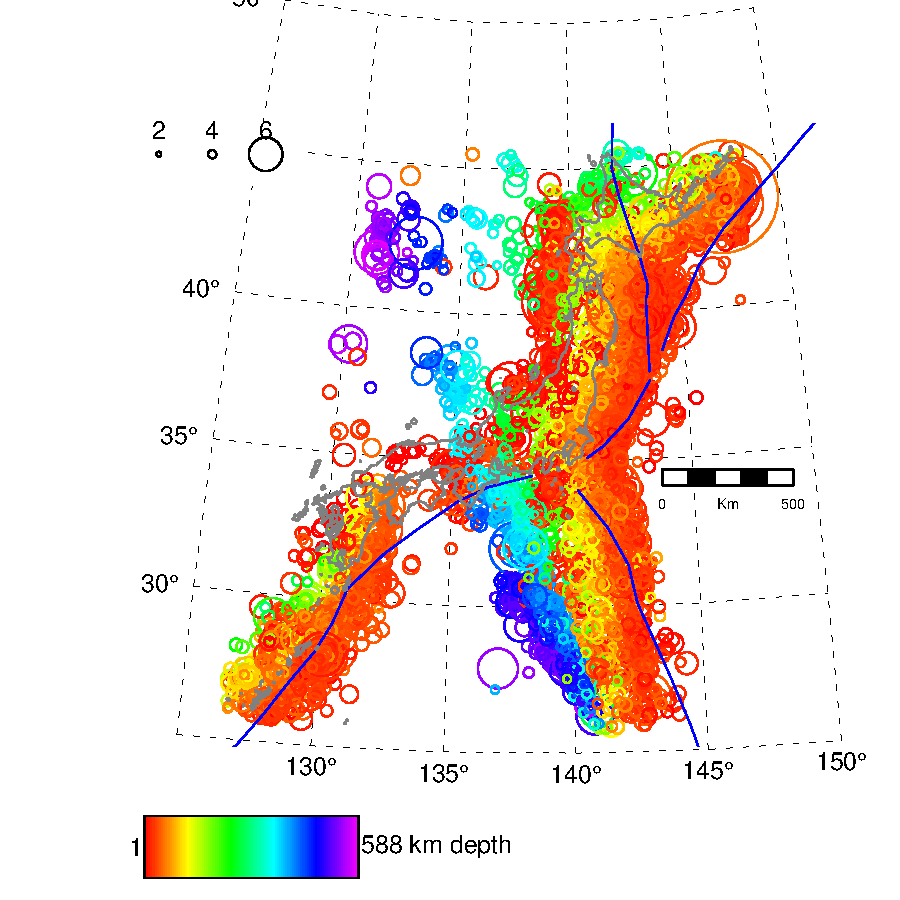
\includegraphics{gmap-022}

Next we can plot this in a slightly different way, using a home grown symbol function.

\begin{Schunk}
\begin{Sinput}
> EXY = GLOB.XY(eqs$lat, eqs$lon, PROJ)
> PLAT = pretty(eqs$lat)
> PLON = pretty(eqs$lon)
> esiz = exp(eqs$m)
> rsiz = RESCALE(esiz, 0.04, 0.2, min(esiz), max(esiz))
> ordsiz = order(rsiz, decreasing = TRUE)
> acol = rcol[ecol]
> plotGEOmapXY(japmap, PROJ = PROJ, SEL = isel, xlab = "", ylab = "", 
     axes = FALSE)
> addLLXY(PLAT, PLON, GRIDcol = "black", LABS = 0, BORDER = 0, 
     PROJ = PROJ)
> pgon(EXY$x[ordsiz], EXY$y[ordsiz], siz = rsiz[ordsiz], col = acol[ordsiz], 
     border = "black", startalph = 60, K = 5, lwd = 0.5, xpd = TRUE)
> plotGEOmapXY(PLATES, PROJ = PROJ, add = TRUE)
> plotGEOmapXY(japmap, PROJ = PROJ, SEL = isel, xlab = "", ylab = "", 
     axes = FALSE, add = TRUE)
> HOZscale(eqs$z, rcol[1:100], units = "km depth", SIDE = 1, s1 = 0.5, 
     s2 = 0.95)
\end{Sinput}
\end{Schunk}
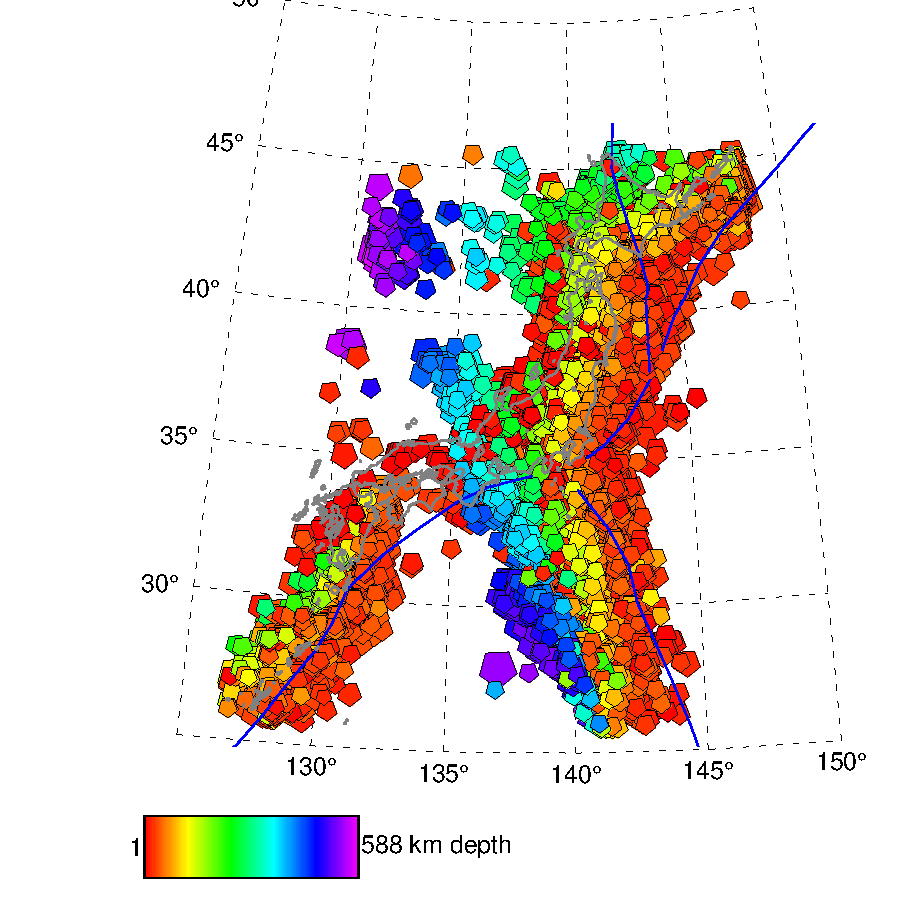
\includegraphics{gmap-023}




\section{Geologic Map Symbols}

Geologic maps are often complex
figures illustrating large amounts of
interconnected information. Numerous line styles
have specific meanings indicating geologic 
structures useful for illustrating relationships
of surface and subsurface features.

Several standard geological symbols are available for plotting
specific  faults on plots.
These can be seen by executing the 
gridded plot of many line dress ups:
\begin{Schunk}
\begin{Sinput}
> GEOsymbols()
\end{Sinput}
\end{Schunk}
\includegraphics{gmap-024}

\end{document}

